\documentclass{../../oss-handout}
\usepackage{enumitem}
\usepackage{tikz}
\usepackage{siunitx}
\usepackage{newtxtext,newtxmath}
\usepackage{bm}
\usepackage{cancel}

\sisetup{
  inter-unit-product=\cdot,
  per-mode=symbol
}
\tikzset{>=latex}

\setlength{\parindent}{0pt}
\setlength{\parskip}{6pt}
\setlength{\headheight}{26pt}

\newcommand{\pic}[2]{\includegraphics[width=#1\textwidth]{#2}}

% Set the page style for the document
\pagestyle{plain}

% Course & handout information
\renewcommand{\institution}{Meritus Academy}
\renewcommand{\coursetitle}{AP Physics C}
\renewcommand{\term}{Updated: Winter 2021}
\title{Solutions to Mechanics Mock Exam}
\author{Dr.\ Timothy Leung}
\date{\today}

\begin{document}
\thispagestyle{title}
\gentitle

\begin{enumerate}[leftmargin=17pt]
\item\textbf{(D)} (A), (B) and (C) are all straight lines which means no
  acceleration. (E) opens downwards which means negative acceleration.

\item\textbf{(D)} Displacement depends only on the initial and final position.

\item\textbf{(B)} Velocity is defined as the rate of change of position (a
  vector) $\dfrac{d\bm{x}}{dt}$ while acceleration is defined as the rate of
  change of of velocity $\dfrac{d\bm{v}}{dt}$ which is also a vector.

\item\textbf{(E)} Both projectiles have the same range, but the one at \ang{60}
  goes higher and therefore stays in the air longer.

\item\textbf{(D)} $t=\SI{2}{\second}$, there is no external net force, so there
  is no acceleration.

\item\textbf{(A)} By definition, equilibrium means no net force (II) acting on
  the object, and by the second law of motion, this means no acceleration (I).
  However, (III) and (IV) are not necessarily true because equilibrium does not
  imply whether it is stationary or in motion. (It depends on the frame of
  reference of the observer.)

\item\textbf{(A)} The initial velocity can be broken down in to the
  vertical ($v_0\sin\theta$) and horizontal ($v_0\cos\theta$) components.
  The horizontal component while vertical acceleration is constant due to
  gravity, $g$. At $P$, there is no vertical velocity.

\item\textbf{(D)} At $Q$, horizontal velocity and acceleration is the same as
  in the previous question, because they are constant. Since $Q$ is at the same
  height as where the rock is thrown, the vertical speed is the same, at
  $v_0\sin\theta$.

\item\textbf{(D)} This is a conservation of momentum problem:
  \begin{equation*}
    m_cv_c=(m_c+m_s)v'\quad\longrightarrow\quad
    v'=\frac{m_cv_c}{m_c+m_s} = \frac{20\times 4.0}{20+5.0}
    =\SI{3.2}{\metre\per\second}
  \end{equation*}

\item\textbf{(A)} None of the statement is true. At the toy reaches the highest
  point, it has zero velocity. We can use the conservation of momentum to
  see that if the 0.02 kg piece moves east, the 0.08 kg piece moves north,
  therefore (I) is not true. The same conservation of momentum will also show
  that the 0.08 kg piece will have a slower horizontal speed than the 0.02 kg
  piece, therefore it lands closer to the launch point, therefore (II) is not
  true. Finally, neither piece has any vertical velocity when the toy splits,
  therefore they both reach the ground at the same time, therefore (II) is not
  true.

\item\textbf{(A)} Before the student jumps off the platform, there is no
  motion, afterwards both are moving, so kinetic energy is not conserved (i.e.\
  the students does positive work). This is analogous to the ``explosion
  problem'' in linear momentum conservation, which there is a net kinetic
  energy after the explosion. Linear momentum is also not conserved
  because the center of mass of the platform is not moving after the student
  jumps off (i.e.\ the axle of the platform exerts an external force as the
  student jumps off), but angular momentum is conserved because the student
  does not exert a torque (nor does the external force from the axle).
  
\item\textbf{(D)} The relationship between period of the simple pendulum and its
  length is related by:
  \begin{displaymath}
    T=2\pi\sqrt{\frac Lg}\quad\longrightarrow\quad
    T^2=\frac{4\pi^2}gL
  \end{displaymath}
  To get a straight graph, plot \fbox{$T^2$ vs.\ $L$}.

\item\textbf{(B)} When a planet orbits the sun, there is a non-zero angular
  momentu. Since gravity is a central force, in that it does not generate any
  torque about the sun, the angular momentum is constant.

\item\textbf{(D)} Two satellites orbiting the same planet must have the same
  constant when using Kepler's third law of planetary motion, i.e.
  \begin{displaymath}
    \frac{T_x^2}{R_x^3}=\frac{T_Y^2}{R_Y^3}\quad\longrightarrow\quad
    \frac{T^2}{R^3}=\frac{(8T)^2}{R_Y^3}\quad\longrightarrow\quad
    R_Y^3=64R^3\quad\longrightarrow\quad R_Y=\boxed{4R}
  \end{displaymath}

\item\textbf{(D)}
  
\item\textbf{(E)} The acceleration of the object is given by the second law of
  motion:
  \begin{displaymath}
    a=\frac Fm=\frac{-3}6t=\frac{-1}2t
  \end{displaymath}
  Integrating in time to get the velocity, and then substituting the initial
  velocity $v_0=\SI{4}{\metre\per\second}$:
  \begin{displaymath}
    v=\frac{-1}2\int tdt=\frac{-1}4t^2+v_0=\frac{-1}4t^2+4
  \end{displaymath}
  Setting $v=0$ and gives $\boxed{t=\SI4{\second}}$.

\item\textbf{(E)} The velocity function is quadratic in time, which means that
  the position function is cubic. There is an initial positive position, which
  means that the $y$-intercept is not zero. (E) is the only graph that fits.
  There is no calculations needed.
  \newpage
  
\item\textbf{(B)} This can be solved by a simple free body diagram of $M_2$:
  \begin{center}
    \begin{tikzpicture}
      \draw(0,0) circle(.05);
      \draw[very thick,->](0,0)--(0,1) node[above]{$T$};
      \draw[very thick,->](0,0)--(0,-1) node[below]{$M_2g$};
      \draw[very thick,->](1,.5)--(1,-.5) node[midway,right]{$a$};
    \end{tikzpicture}
  \end{center}
  Using the second law of motion:
  \begin{displaymath}
    \sum F=ma\quad\longrightarrow\quad
    M_2g-T=M_2(0.6g)\quad\longrightarrow\quad T=\boxed{0.4M_2g}
  \end{displaymath}

\item\textbf{(D)} The weight $M_2g$ is the only force that causes motion, so
  \begin{displaymath}
    \sum F=ma\quad\longrightarrow\quad
    M_2g=(M_2+M_1)(0.6g)\quad\longrightarrow\quad
    0.4M_2g=0.6M_1g\quad\longrightarrow\quad
    \frac{M_2}{M_1}=\boxed{1.5}
  \end{displaymath}
  The most common mistake is to reverse the ratio.

\item\textbf{(E)} We can do a quick energy conservation equation:
  \begin{displaymath}
    \cancel{K} +\cancel{U_{g1}} +\cancel{U_{g2}}+\cancel{U_e}+
    \underbrace{W_f}_{<0}=
    \cancel{K'}+\cancel{U_{g1}'}+\underbrace{U_{g2}'}_{<0}+U_e'
  \end{displaymath}
  Since friction does negative non-conservative work on the system, the gain
  in elastic potential energy must be less than the loss in gravitational
  potential energy.
  
\item\textbf{(C)} After the block stops, the forces on Block 1 must be balanced.
  
\item\textbf{(C)} The area under the force vs.\ time graph is the impuslse,
  which is also the change in momentum. In this case, the area is in the form
  of a triangle, with an area of
  \begin{equation*}
    \Delta p = I = \boxed{\frac12 Ft}
  \end{equation*}

\item\textbf{(E)} This is a simple center of mass calculation. If the distance
  between the moon and the planet is $r_A$, then the CM would be located at
  $\dfrac{m}{50m}r_A=\dfrac1{50}r_A$ from the planet, or
  $\boxed{\dfrac{49}{50}r_A}$ from the moon.
 
\item\textbf{(B)} The angular momentum of the moon about the planet is constant
  because gravity does not generate a torque about the planet. Therefore
  \begin{displaymath}
    L=r_Amv_0=r_Bm(5v_0)\quad\longrightarrow\quad
    r_B=\boxed{\frac15r_A}
  \end{displaymath}

\item\textbf{(D)} There is no need to do calculations here, but it is worthwhile
  to see how angular acceleration changes as the bar rotates. The torque
  generated by the weight is
  \begin{displaymath}
    \tau=mg\sin\theta=I\alpha
  \end{displaymath}
  This means that angular acceleration $\alpha$ increases as the bar rotates,
  reaching \emph{maximum value} at $\theta=\ang{90}$. While $\theta$ is not
  linear with $t$, (D) is only one graph that shows both an increasing
  $\alpha(y)$ as well as a one with a \emph{maximum} at the end (i.e.\ zero
  slope).
  
\item\textbf{(E)} The angular velocity function can be obtained simply by
  integrating the angular acceleration function\ldots except we don't have to
  do that! Since we know that angular acceleration is maximum at the end,
  the slope of the angular velocity graph must also have the steepest positive
  slope. Graph (E) is the only one that fits that.

\item\textbf{(C)} As the stone falls, it is subjected to a constant
  gravitational force $mg$, which exerts a constant torque about point $P$.
  Therefore the angular momentum about $P$ increases linearly.

\item\textbf{(C)} The table shows that the force is related to the spring
  displacement by $F=x^3$. Integrating this from 0 to 3 gives the potential
  energy of:
  \begin{displaymath}
    U=\int_0^3 Fdx=\int_0^3 x^3dx = \frac14x^4\Biggr|^3_0 = \frac{81}4
  \end{displaymath}

\item\textbf{(B)} In such a spring, the velocity function will be given by
  \begin{displaymath}
    v(t)= A\omega\cos(\omega t)
  \end{displaymath}
  If you have forgotten, you can differentiate the position function
  $x(t)=A\cos(\sin t)$. It does not matter if you use $\cos(\omega t)$ or
  $\sin(\omega t)$. The kinetic energy is given by:
  \begin{displaymath}
    K(t)=\frac12mv^2=\frac12{A^2}
    \underbrace{m\omega^2}_{=m\left(\sqrt{\frac km}\right)^2=k}
    \cos^2(2\omega t)=\boxed{\frac12kA^2\cos^2(\omega t)}
  \end{displaymath}

\item\textbf{(C)} The work done by the external force can be found by
  integrating the force by displacment $dx$:
  \begin{displaymath}
    W= \int_D^0 Fdx = \int_D^0 (-ax+bx^2)dx
    =\left(\frac{-1}2ax^2+\frac13bx^3\right)\Biggr|^0_D
    =\boxed{\frac12aD^2-\frac13bD^3}
  \end{displaymath}
  \newpage
  
\item\textbf{(A)} The forces acting on the ladder are:
  \begin{center}
    \begin{tikzpicture}[scale=.9]
      \draw[very thick](0,5)--(0,0)--(4,0);
      \begin{scope}[rotate around = {atan(.75):(3,0)}]
        \draw[fill=gray,very thick](3,0) rectangle (3.2,5);
        \fill[red!70!black](3.1,2.5) circle(.08);
        \draw[red!70!black,ultra thick,->,rotate around={-atan(.75):(3.1,2.5)}]
        (3.1,2.5)--(3.1,1) node[left]{$W$};
      \end{scope}
      \fill[red!70!black](3,0) circle(.08);
      \draw[red!70!black,ultra thick,->] (3,0)--(3,1.5) node[right]{$N_1=W$};
      \draw[red!70!black,ultra thick,->] (3,0)--(2,0) node[below]{$f$};
      \fill[red!70!black](0,4) circle(.08);
      \draw[red!70!black,ultra thick,->] (0,4)--(1,4) node[right]{$N_2=f$};
    \end{tikzpicture}
  \end{center}
  The normal force exerted by the floor is equaled to the weight of the ladder,
  i.e. $N_1=W$, since they are the only vertical forces.
  
\item\textbf{(E)} In order for the ladder to be static, the sum of all the
  torques must be zero. The net torque can be calculated \emph{anywhere}, but
  for this problem it is easiest to calculate it at the center of mass. The
  normal force at the wall must be equal to static friction, $N_2=f$, because
  these are the only two horizontal forces. The torques are:
  \begin{align*}
    \sum\tau=-f\frac L2\sin\theta-f\frac L2\sin\theta+W\frac L2\cos\theta&=0\\
    W\cos\theta&=2f\sin\theta\\
    f&=\frac W2\frac{\cos\theta}{\sin\theta}=\boxed{\frac W2\cot\theta}
  \end{align*}

\item\textbf{(E)} When the spring is cut in half, it would take twice as much
  force to stretch it by the same distance, therefore the spring constant
  increases by a factor of 2, i.e.\ $\boxed{2k}$.

\item\textbf{(C)} This planet has half the radius of earth, $r'=\frac12 r$, but
  the weight of the astronaut is also twice that of Earth, i.e.\ $g'=2g$. Using
  the definition of gravitational field, we find the mass of the planet is half
  that of Earth:
  \begin{equation*}
    g'=\frac{GM}{r'^2}\quad\longrightarrow\quad
    (2g)=\frac{GM'}{(\frac12r)^2}\quad\longrightarrow\quad
    2g=\frac{4GM'}{r^2}\quad\longrightarrow\quad
    M'=\frac{gr^2}{2G}=\frac12M
  \end{equation*}
  The escape speed of any small object from a much larger planet is given by
  \begin{equation*}
    v_\text{esc}=\sqrt{\frac{2GM}{r}}
  \end{equation*}
  In this case, decreasing the mass by half, while decreasing the radius by half
  does not change the escape velocity.
\item\textbf{(E)} The gravitational force on $m$ is linearly proportional
  to the distance from the center $F_g=\dfrac{GMm}{R^3}r$, therefore the kinetic
  energy at the center is given by:
  \begin{equation*}
    W=K=\int F_gdr=\frac{GMm}{R^3}\int_0^R rdr=
    \frac{GMm}{2R^3}r^2\Biggr|^R_0=\boxed{\frac{GMm}{2R}}
  \end{equation*}
  Which is (III). However, given that the gravitational field at the surface
  $g=\dfrac{GM}{R^2}$, the expression for kinetic energy can be written as
  \begin{equation*}
    K=\frac{GMm}{2R}=\frac{GMm}{R^2}\frac R2=\boxed{\frac12mgR}
  \end{equation*}
\end{enumerate}
\end{document}
